\section{Theorie}
\label{sec:Theorie}

\subsection{Das Geiger-Müller-Zählrohr}
Das verwendete Zählrohr besteht, wie in Abbildung \ref{fig:GMZ} dargestellt, aus einem Zylindermandel aus Stahl, der als Kathode dient und einem Anodendraht. Zwischen Mantel und Draht wird eine Spannung von $U= 300 - 2000 \text{V}$ angelegt. Das dadurch entstehende elektrische Feld in Abhängigkeit vom Abstand $r$ zur Zählrohrachse ist gegeben durch
\[
E(r)=\frac{U}{r\ln\left(\frac{r_.K}{r_.A}\right)},
\]
wobei $r_.K$ und $r_.A$ die Radien des Zählrohrmantels bzw. des Drahtes sind.\newline
\begin{figure}
\centering
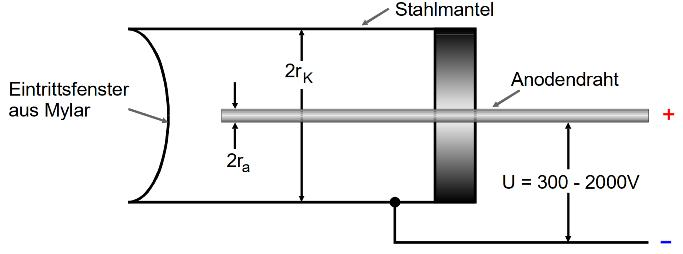
\includegraphics[scale=0.5]{content/images/aufbau1.jpg}
\caption{Aufbau eines Geiger-Müller-Zählrohrs \cite{V703}.}
\label{fig:GMZ}
\end{figure}
Die eine Seite des Zylinders ist geschlossen auf der anderen befindet sich ein aus Mylarfolie bestehendes Endfenster, durch das die Teilchen eindringen können. Das Zählrohrinnere ist mit einem Gasgemisch gefüllt.
\subsection{Totzeit eines Geiger-Müller-Zählrohres}
